\documentclass[10pt]{article}
\usepackage[a4paper,margin=1.6cm,top=1.3cm,bottom=1.3cm]{geometry}
\usepackage[T1]{fontenc}
\usepackage{lmodern}
\usepackage{microtype}
\usepackage{booktabs}
\usepackage{graphicx}
\usepackage{enumitem}
\usepackage{xcolor}
\usepackage[colorlinks=true,linkcolor=black,citecolor=black,urlcolor=blue]{hyperref}
\setlist{nosep,leftmargin=1.2em,topsep=1pt}
\setlength{\parindent}{0pt}
\setlength{\parskip}{3pt}
\pagestyle{empty}
\newcommand{\head}[1]{\par\smallskip{\large\bfseries #1}\par}
\newcommand{\sect}[1]{\par\smallskip{\bfseries\color{black!80} #1}\par}

\begin{document}
\head{Idea 3 PoC --- Are record earnings a reference point?}
\textit{Proof of concept, October 2026. Code: \texttt{idea03\_record\_earnings/run.py}.}

\sect{Question and design}
Price anchors such as the 52-week high shape how investors react to news (George and Hwang, 2004; Li and Yu,
2012). Is a firm's \emph{record} earnings an anchor too? For each quarterly report (2005--2020) we compute the
distance to the record:
$r=(\mathit{TTM}_{\mathrm{new}}-\max \mathit{TTM}_{\mathrm{earlier}})/\sigma$. Trailing-twelve-month (TTM) EPS is the
sum of the last four standalone quarters, and $\sigma$ is the SD of the firm's past SRW errors. At least eight
earlier TTM values are required, and exact ties with the old record are dropped. Firms just above zero set a new
record; firms just below narrowly miss it. We estimate local-linear regressions around $r=0$, controlling for the
surprise with separate slopes for good and bad news, with SEs clustered by month. We test for a \emph{jump} (a
premium for the record itself) and a \emph{kink} (a steeper response to how far the firm moves past its record). We
check balance and bunching, and run placebo cutoffs. The sample has 95{,}567 reports, 20\% of them new records.

\begin{center}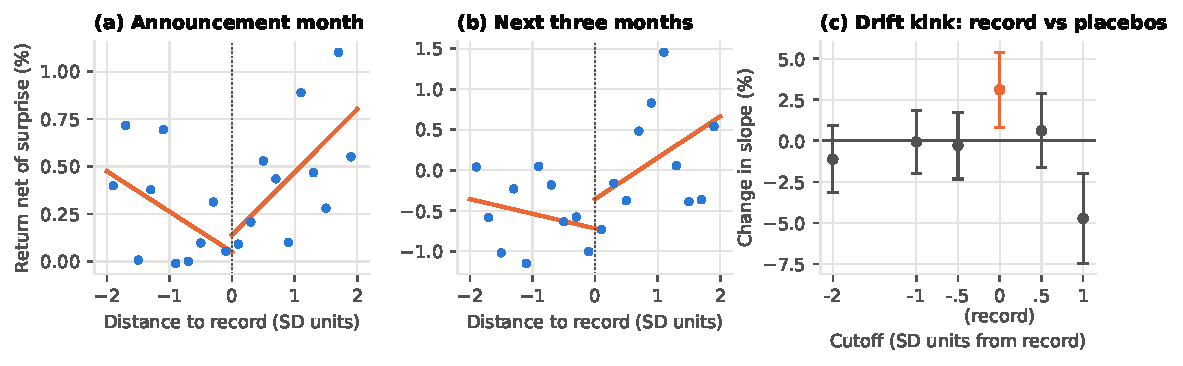
\includegraphics[width=0.97\textwidth]{results/fig_main.pdf}\end{center}

\begin{center}\small
\begin{tabular}{lcccc}
\toprule
At the record ($r=0$) & \multicolumn{2}{c}{Announcement month} & \multicolumn{2}{c}{Months $+1..+3$}\\
 & $h=1$ & $h=2$ & $h=1$ & $h=2$\\
\midrule
Jump (\%) & $-0.09$ ($-0.3$) & 0.07 (0.3) & 0.34 (0.7) & 0.19 (0.6)\\
Kink: change in slope (\% per SD) & 1.07 (1.5) & 0.75 (2.7) & 3.12 (2.7) & 1.45 (2.8)\\
\bottomrule
\end{tabular}
\hspace{0.6em}
\begin{tabular}{ll}
\toprule
Check & Estimate ($t$)\\
\midrule
Placebo drift kinks at $-2$, $-1$, $-0.5$, $+0.5$ & all $|t|\leq1.1$\\
Placebo drift kink at $+1$ & $-4.7$ ($-3.4$)\\
Balance: surprise, momentum, pre-return & $t$ = 0.9, 1.4, 0.9\\
Balance: size & \textbf{$t$ = 3.3}\\
Bunching just above the record & +3.3\% (1.2)\\
Benchmark: jump at SUE $=0$ ($h=2$) & 0.30\% (1.7)\\
\bottomrule
\end{tabular}\\[2pt]
{\footnotesize $t$-statistics in parentheses. $h$ is the bandwidth in SD units (triangular kernel). Returns are
size-adjusted.}
\end{center}

\sect{Findings}
\begin{itemize}
\item \textbf{No premium for the record itself, and no manipulation.} Returns do not jump when a firm just beats its
  record, and there is no bunching of reports just above it. Firms do not seem to manage earnings to set records.
\item \textbf{But crossing the record changes how news is priced.} Below the record, returns net of the surprise do not
  rise with the distance to it (if anything they fall). Above it, they rise steeply, and most of the extra response arrives over the
  \emph{next three months} (slope change of 1.5--3.1\% per SD, $t\approx2.7$). Placebo cutoffs below the record show
  no such kink. This is the pattern of an anchor: investors underreact to earnings news that pushes through the
  record, and prices catch up later, much like the 52-week-high effect but in earnings.
\item \textbf{Caveats.} The effect is local. The response is steep just above the record and flattens beyond about
  one SD, hence the negative placebo kink at $+1$. Firms just above the record are also somewhat larger ($t=3.3$).
  Monthly returns limit power: even the classic ``beat last year'' threshold is only marginal here.
\end{itemize}

\sect{Assessment and next steps}
More promising than expected: a new anchor (the earnings record) with an underreaction pattern, robust to an
asymmetric surprise control and placebo cutoffs, but fragile in its shape. Next steps: (i) daily returns and
announcement-window CARs; (ii) control for size and growth persistence (how many quarters TTM has risen) to separate
anchoring from rational learning about growth; (iii) a portfolio test (buy new-record firms after the announcement);
(iv) use media headlines that mention ``record profit'' to measure salience directly.
\end{document}
